\chapter{Message Construction}
An AYDP message is constructed from three basic components; a header, a data section, and a checksum. The checksum at the end of each sentence is a single byte which is the XOR of all of the bytes in the sentence (excluding itself). This checksum byte is only intended to allow the recipient to ensure that the message is complete, not to re-build any missing data.

\begin{figure}[H]
  \centering
  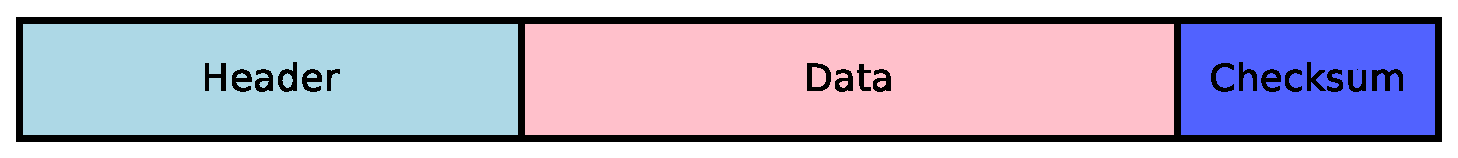
\includegraphics[width=1.0\textwidth]{Figures/protocolBasicLayout.eps}
  \label{figure:msg:basicProto}
  \caption{Basic protocol layout}
\end{figure}

The header is 27 bytes long and contains the message type and length as shown in table \ref{table:msg:header}.

\begin{table}[H]
  \centering
  \begin{tabular}{ c c c c }
  Byte &          Content    & Data Type & Length  \\
       &                     &           & (bytes) \\
\hline
   1   &  Start (0xFF)       &   uint8   &    1    \\
   2   &  Message Type       &   uint8   &    1    \\
   3   &  Message Length     &   uint32  &    4    \\
   7   &  Seconds from epoch &   int64   &    8    \\
   19  &  Milliseconds into current second & int64 & 8 \\
  \end{tabular}
  \caption{Header Contents}
  \label{table:msg:header}
\end{table}

\input{section.tex} 